\documentclass[conference]{IEEEtran}
\IEEEoverridecommandlockouts
% The preceding line is only needed to identify funding in the first footnote. If that is unneeded, please comment it out.
\usepackage{cite}
\usepackage{amsmath,amssymb,amsfonts}
\usepackage{algorithmic}
\usepackage{graphicx}
\usepackage{textcomp}
\usepackage{xcolor}
\usepackage[settings]{markdown}

\def\BibTeX{{\rm B\kern-.05em{\sc i\kern-.025em b}\kern-.08em
    T\kern-.1667em\lower.7ex\hbox{E}\kern-.125emX}}
\begin{document}

\title{
Robocup Project Report
}

\author{\IEEEauthorblockN{Aron Arany-Takacs}
\IEEEauthorblockA{\textit{Electrical Engineering and Computer Science} \\
\textit{University of Ottawa}\\
Ottawa, Canada \\
aaran043@uottawa.ca}
\and
\IEEEauthorblockN{Bardia Parmoun}
\IEEEauthorblockA{\textit{Systems and Computer Engineering} \\
\textit{Carleton University}\\
Ottawa, Canada \\
bardiaparmoun@cmail.carleton.ca}
\and
\IEEEauthorblockN{Dylan Leveille}
\IEEEauthorblockA{\textit{Systems and Computer Engineering} \\
\textit{Carleton University}\\
Ottawa, Canada \\
dylanleveille@cmail.carleton.ca}
}

\maketitle

\begin{abstract}
\texttt{JASON} is a Java-based interpreter for an extended version of \texttt{AgentSpeak}. In this work, we make use of \texttt{JASON} to prescribe unique beliefs, desires, and intentions to different player types in a \texttt{Robocup} soccer team. Specifically, the player types that have been created using \texttt{JASON} are \textit{Goalie}, \textit{Defender}, and \textit{Attacker}. The primary contribution of this work is the creation of distinct player types that possess a heightened sense of spatial awareness (e.g., using player and ball locations) to allow for better positioning during play. Such positioning allows the players to be better prepared against opponent strategies and increase their overall cooperation.
\end{abstract}


\section{Program Design}

This section describes the design of our program. Our \texttt{Robocup} team is composed of five players: two \textit{Attackers}, two \textit{Defenders}, and one \textit{Goalie}. Each player type is defined in their respective \texttt{.asl} file within the \texttt{resources} folder. This separation enables unique beliefs, desires and intentions for each player type. 

Figure~\ref{fig:robocupDesign} provides an overview of the process followed by our program when initializing a new \texttt{Robocup} player.  When starting a player (through RobocupAgent.java), depending on the player type provided as input for the player, the corresponding player type enum is sent to the Brain.java constructor. Brain.java uses this enum to identify the \texttt{.asl} file to be used for the player. Following this, it creates a \texttt{JASON} agent from the specification in this \texttt{.asl} file. Once finished, RobocupAgent.java will start the Brain.java thread. As Brain.java extends \texttt{JASON}'s AgArch class, it will perceive and interact with the \texttt{Robocup} environment. 

\begin{figure}[ht!]
    \centering\centerline{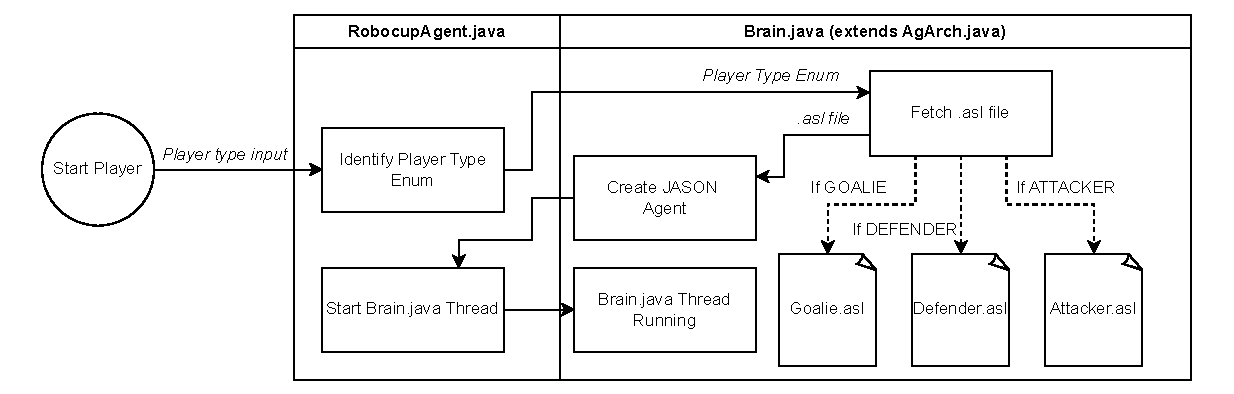
\includegraphics[width=.5\textwidth]{Figures/DesignWorkflow.pdf}}
    \caption{An overview of the workflow for initializing \texttt{Robocup} player.}
    \label{fig:robocupDesign}
\end{figure}

Figure~\ref{fig:robocupExecution} provides an overview of the process followed by our program during the execution of a \texttt{Robocup} player. When the Brain.java thread begins execution, depending on its player type, it will place the player in its respective playing position on the field. While the thread is running, a \texttt{JASON} reasoning cycle will be requested. The \texttt{JASON} transition system (specified in TransitionSystem.java) will request that the environment be perceived. To perceive the environment, the \texttt{Perceive} method was overridden in Brain.java. In this method, we perceive various environmental properties to create logical literals that serve as perceivable beliefs for the player. These literals are passed to the \texttt{JASON} transition system. 

Using these perceivable beliefs, certain actions may be considered for certain steps in the intentions reasoned by \texttt{JASON}. If an action is required, the action is taken in the overridden \texttt{act} method of Brain.java. Specifically, in this method, based on a text-formatted action provided by \texttt{JASON}, an actual action corresponding to this string is taken by the player. When the reasoning cycle ends, if the player has performed an action during the reasoning cycle, the player will go to sleep for the duration of a \texttt{Robocup} clock cycle to avoid sending more than one player action to the \texttt{Robocup} server. When the sleep is finished, another \texttt{JASON} reasoning cycle will be requested. Similarly, if no action was taken during the reasoning cycle, a new \texttt{JASON} reasoning cycle will be requested.

   

\begin{figure}[ht!]
    \centering\centerline{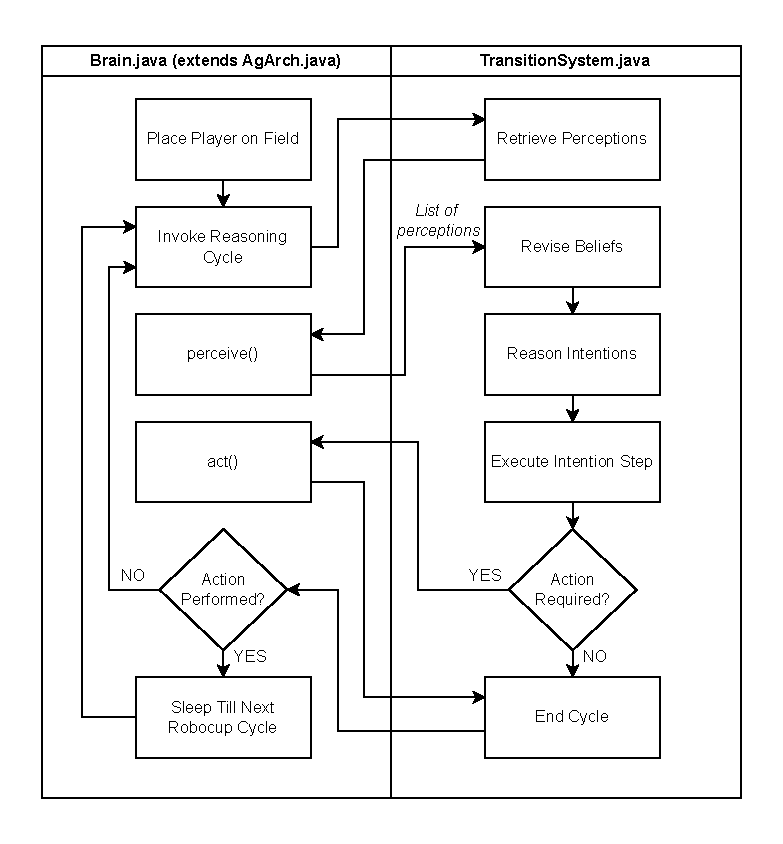
\includegraphics[width=.35\textwidth]{Figures/ExecutionWorkflow.pdf}}
    \caption{An overview of the workflow during execution of a \texttt{Robocup} player.}
    \label{fig:robocupExecution}
\end{figure}
 





\section{Player Functionalities and Expected Behaviour}
In this section, we describe each player type's functionality and expected behaviour. 

\subsection{Goalie}\label{AA}
The goalie's \texttt{JASON} specification is found in the \texttt{goalie.asl} file. Fundamentally, the goalie should not move away from its net unless a ball is approaching and must be caught. As a result, in this file, notice that the goalie has an initial goal of \texttt{!wait}. With this goal, it simply attempts to find the ball and keep track of its direction. When the ball moves away from the center, and passes the center-top (\texttt{flag c t}) and center-bottom (\texttt{flag c b}) flags at certain angles, the goalie will move to different positions to better protect its goal. Specifically, there are five possible positions for the goalie: \textit{center}, \textit{right}, \textit{veryRight}, \textit{left}, and \textit{veryLeft}. The goalie will start in the \textit{center} position (explaining its initial belief, \texttt{in\_centre\_position}). When the ball has passed the center-top or centre-bottom flags at an angle of 5 degrees, it will move into the \textit{right} or \textit{left} position respectively (depending on the goalie's side of the field). Similarly, when the ball has passed these flags at an angle of 20 degrees,   it will move into the \textit{veryRight} or \textit{veryLeft} position respectively (again, depending on the goalie's side of the field). Figure~\ref{fig:goaliePositions} labels and visualizes each possible goalie position. 

\begin{figure}[ht!]
    \centering\centerline{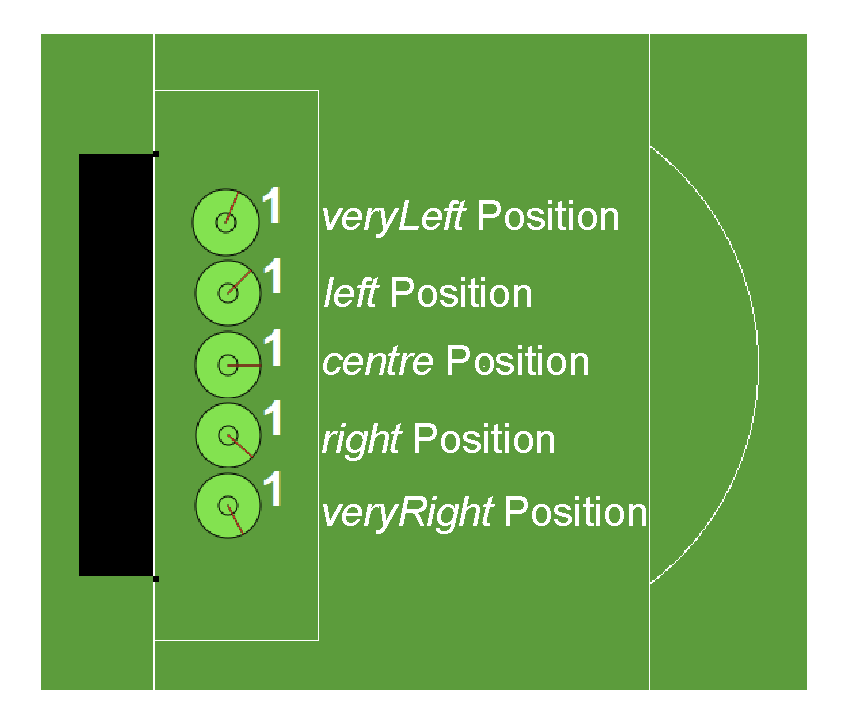
\includegraphics[width=.3\textwidth]{Figures/GoaliePositions.pdf}}
    \caption{A visualization of all possible goalie positions.}
    \label{fig:goaliePositions}
\end{figure}

The goalie will wait in these positions until the ball is within a distance of 10 meters, and the ball is at a minimum angle of 7.5 degrees from the goalie. If the angle is too large, the goalie will attempt to turn to the ball to close the angle. When both of these conditions are met, the goalie will dash to the ball and attempt to catch it. If caught, the goalie will pass the ball to one of its teammates. Specifically, if there are no opponents between the goalie and the furthest defender on the team, the ball will be passed to that defender. Similarly, if there are no opponents between the goalie and the nearest attacker on the team, the ball will be passed to that attacker. If the ball cannot be passed to either of these players, it will be kicked to the right at a 45-degree angle from the center, near the center-top flag (\texttt{flag c t}). When the ball is no longer within 10 meters of the goalie, the goalie will reset to its \textit{centre} position.

\subsection{Defender}\label{AA}
The defender's \texttt{JASON} specification is found in the \texttt{defender.asl} file. The defender will only have 3 main goals throughout the game. Its first goal, \texttt{!wait}, has to do with its main loop which is very similar to Krislet's behaviour. In other words, the defender first 
the player attempts to locate the ball through 40-degree turns. When found, it will continuously align with the ball. When the ball reaches a close distance (1 m) to the defender, the defender checks if it can view the opposing goal. If the goal is visible, it attempts a kick towards that goal. If not, it will look for an attacker on its team, and attempt a pass to that attacker. If the latter cannot be found, it will attempt to look for attackers on its team through 40-degree turns.

A key component of the defender is its ability to ensure that it remains in its operating zone. As a result, its second \texttt{JASON} goal is to return to its home zone once it exits it. To achieve this, a defender will repeatedly scan flags around the field and calculate their distance from each. On each side of the field, the defenders use that field's goal flag along with its corner flags. If the defender's distance to any of its home flags is below a threshold (18 m or 35\% of the field length), it registers \texttt{in\_home\_zone} belief. Similarly, if the defender's distance from any of its opponent flags is below a threshold, it registers a \texttt{~in\_home\_zone} belief. When the defender is not close to any of the flags, it will not know anything about its home zone. 

Figure~\ref{fig:defenderZones} illustrates these zone calculations for both the attacker and the defender.

\begin{figure}[ht!]
    \centering\centerline{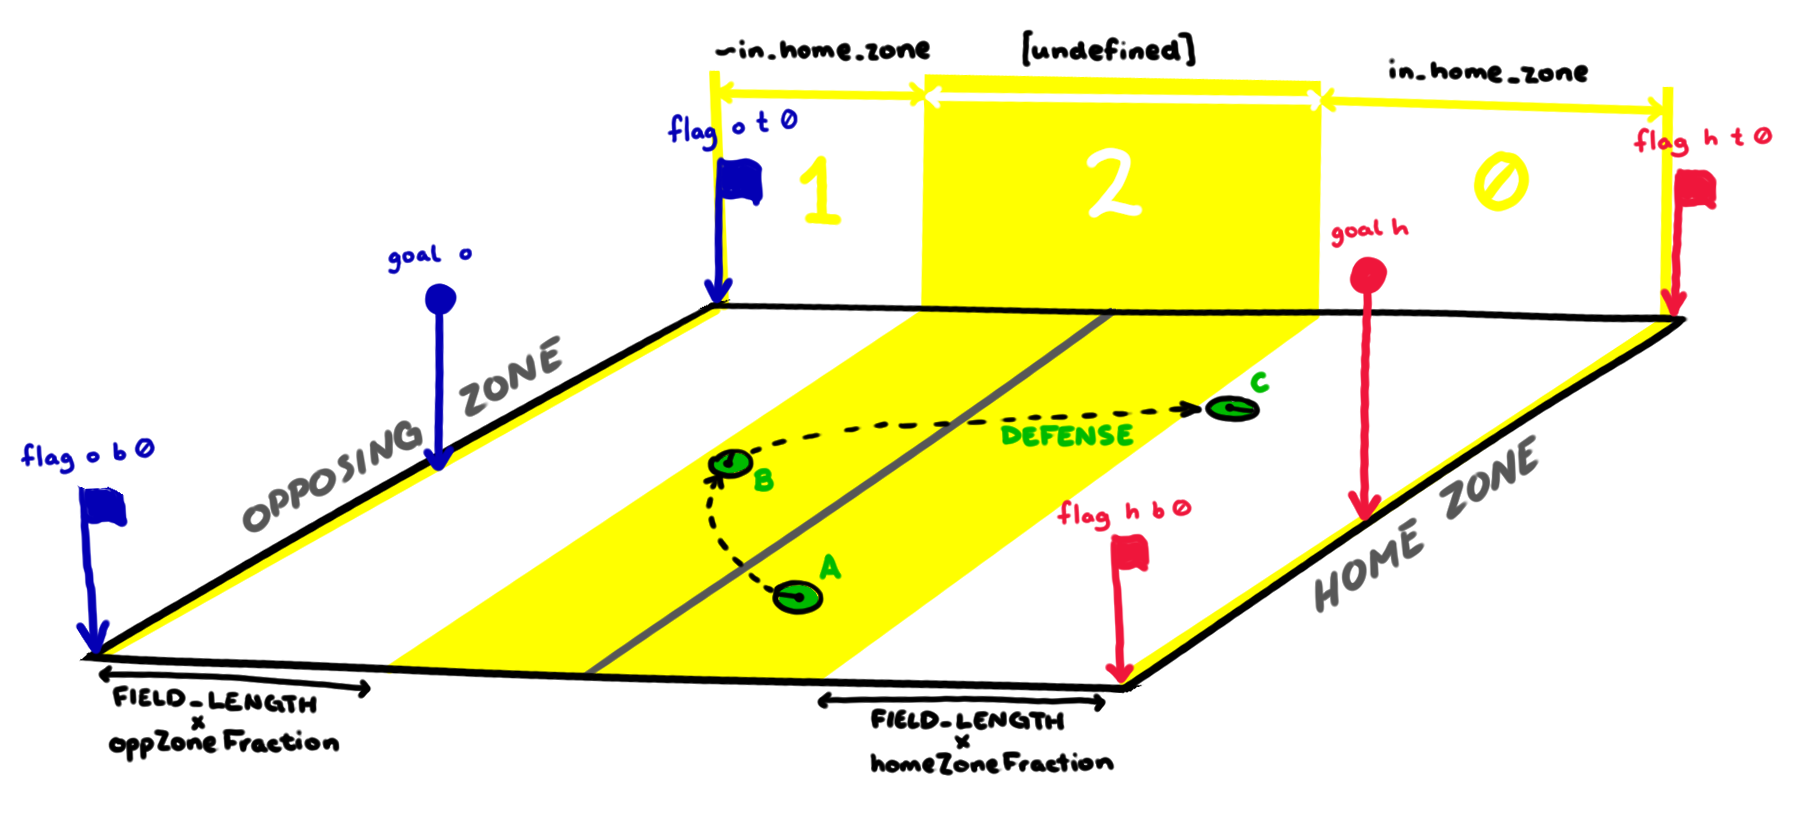
\includegraphics[width=.5\textwidth]{Figures/zone_demonstration.png}}
    \caption{A visualization of the zone belief interpretations performed by the defensive agent.}
    \label{fig:defenderZones}
\end{figure}

Note that each defender has a designated flag assigned to them, at an angle of $\pm$ 40 degrees from the center of the goals. Upon returning to their home zone, the defenders align themselves with their designated flag. This ensures that they will return at a specific angle, and thus be spread out.

Finally, the defenders need to cooperate properly with the goalie. As such, the defender's third goal is to ensure that they only go for the ball when it is not in the possession of the goalie. To achieve this, the defender uses its distance and relative angle with the goalie and the ball to estimate the distance between the goalie and the ball. It then checks this distance against a threshold (the same threshold used by the goalie to catch the ball) to see if the goalie is going to attempt to catch the ball. An example of this is shown in Figure~\ref{fig:estimateGoalieDistance}. The variables in the figure are defined as follows: 
\begin{itemize}
\item \texttt{d\_ball}: defender's distance with the ball.
\item \texttt{d\_goalie}: defender's distance with the goalie.
\item \texttt{d\_goalie\_to\_ball}: goalie's distance with the ball.
\item \texttt{ball\_angle}: defender's angle with the ball.
\item \texttt{goalie\_angle}: defender's angle with the goalie.
\end{itemize}

Using \textit{cosine's law}, \texttt{d\_goalie\_to\_ball} can be calculated as follows:

\[
\resizebox{\columnwidth}{!}{$
\begin{aligned}
    \text{angle\_in\_between} &= \text{goalie\_angle} - \text{ball\_angle} \\
    \text{d\_goalie\_to\_ball} &= 
    \sqrt{d_{\text{ball}}^2 + d_{\text{goalie}}^2 - 2 \cdot d_{\text{ball}} \cdot d_{\text{goalie}} \cdot \cos(\text{angle\_in\_between})}
\end{aligned}
$}
\]

\begin{figure}[ht!]
    \centering\centerline{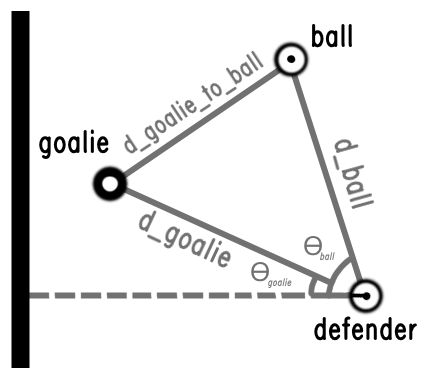
\includegraphics[width=.25\textwidth]{Figures/triangulation_defender_goalie.png}}
    \caption{A visualization of how the defender estimates the distance between the goalie and the ball.}
    \label{fig:estimateGoalieDistance}
\end{figure}

Once the defender has concluded that the goalie has the ball, it checks to see if it is too close to the goalie. If it considers itself to be too close (less than 10 m) to the goalie, it heads back toward the center of the field at the same angle that it uses for its designated flag. This ensures that the defenders will be spread out if the goalie catches the ball and performs a free kick. Once the defenders are far from the goalie, they will wait until the goalie has released possession of the ball.

\subsection{Attacker}\label{AA}
The offensive player agent (defined by \texttt{attacker.asl}) can be considered an inverse of the defender agent, where similar beliefs are interpreted to keep the player in the oppositional zone. Whereas the defense agents are soft-bound to play in the home zone, the offensive players will relocate to forward positions, defined by aligning themselves with a specified offset and running to the area of the field where the \texttt{in\_home\_zone} belief is added to the \texttt{JASON} agent. This behavior is only enacted when the \texttt{JASON} framework believes \texttt{not(ball\_seen)}, and the offensive player can still play defense within a certain range, if necessary. In order to prevent over-aggression by means of triggering the offside penalty, the ability to detect offside conditions was integral to the pacing of the offensive agent. To this end, a triangulation algorithm was implemented to update the agent's beliefs (\ref{fig:offsideTriangulation}).

%[Fig X: Triangulation chart]
\begin{figure}[ht!]
        \centering\centerline{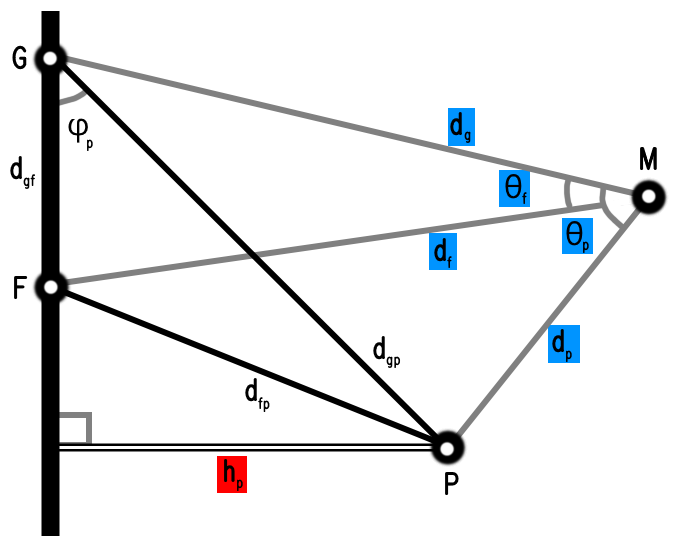
\includegraphics[width=0.25\textwidth]{Figures/triangulation.png}}
        \caption{Triangulation scheme used to detect offside conditions. Law of Cosines are applied to retrieve the distance from the opposition line $h_p$}
        \label{fig:offsideTriangulation}
\end{figure}

The agent will iterate over all visible enemy players, then compare them with the perceived \texttt{h} distance of the observed ball. If the ball is located behind all enemies (excluding the opposing Goalie), the agent will run at a reduced rate instead of a full sprint, usually ensuring the ball will be returned to the possession of the opposition, avoiding an offside foul. Note that the previously calculated zone beliefs are applied to the detection of offsides, as they can only occur in the oppositional zone.

\section{Agent Software Design}
When implementing the BDI logic using \texttt{JASON}, careful management of active beliefs and their catchment was essential to maintaining defined agent behavior. In order to orchestrate the goal transitions of the agent, we modelled a hub-and-spoke flow to triggering events, centralizing the decision-making on the \texttt{!wait} event, with "spokes" being extant subroutine-style plans that handle a certain aspect of agent behavior. These branches tend to serve \texttt{!wait} once the desired behavior is complete. The goalie agent, due to advanced positioning mechanics, has more extant branching involved, but the return-to-idle behavior remains consistent.

\section{Running the JasonBDI Soccer Agent}
If you are on Windows simply double-click on the \texttt{TeamStart.bat} file to run two teams with the \texttt{JASON} player types described in this report. Similarly, if you are on a \texttt{UNIX} machine you can run the shell script using: \begin{markdown}
```
$ ./TeamStart
```
\end{markdown}
\noindent For the initialization of a single team (5 players), the batch script \texttt{HalfTeamStart.bat} Windows and \texttt{HalfTeamStart.sh} can be run instead. These scripts are designed to allow for running the players against another RoboCup Team.




%%% Removes the rest of the template
\iffalse
%\iftrue

\section{Figures and Tables (TEMPLATE FROM HERE)}
\paragraph{Positioning Figures and Tables} Place figures and tables at the top and 
bottom of columns. Avoid placing them in the middle of columns. Large 
figures and tables may span across both columns. Figure captions should be 
below the figures; table heads should appear above the tables. Insert 
figures and tables after they are cited in the text. Use the abbreviation 
``Fig.~\ref{fig}'', even at the beginning of a sentence.

\begin{table}[htbp]
\caption{Table Type Styles}
\begin{center}
\begin{tabular}{|c|c|c|c|}
\hline
\textbf{Table}&\multicolumn{3}{|c|}{\textbf{Table Column Head}} \\
\cline{2-4} 
\textbf{Head} & \textbf{\textit{Table column subhead}}& \textbf{\textit{Subhead}}& \textbf{\textit{Subhead}} \\
\hline
copy& More table copy$^{\mathrm{a}}$& &  \\
\hline
\multicolumn{4}{l}{$^{\mathrm{a}}$Sample of a Table footnote.}
\end{tabular}
\label{tab1}
\end{center}
\end{table}

\begin{figure}[htbp]
\centerline{\includegraphics{fig1.png}}
\caption{Example of a figure caption.}
\label{fig}
\end{figure}

Figure Labels: Use 8 point Times New Roman for Figure labels. Use words 
rather than symbols or abbreviations when writing Figure axis labels to 
avoid confusing the reader. As an example, write the quantity 
``Magnetization'', or ``Magnetization, M'', not just ``M''. If including 
units in the label, present them within parentheses. Do not label axes only 
with units. In the example, write ``Magnetization (A/m)'' or ``Magnetization 
\{A[m(1)]\}'', not just ``A/m''. Do not label axes with a ratio of 
quantities and units. For example, write ``Temperature (K)'', not 
``Temperature/K''.

\section*{Acknowledgment}

The preferred spelling of the word ``acknowledgment'' in America is without 
an ``e'' after the ``g''. Avoid the stilted expression ``one of us (R. B. 
G.) thanks $\ldots$''. Instead, try ``R. B. G. thanks$\ldots$''. Put sponsor 
acknowledgments in the unnumbered footnote on the first page.

\section*{References}

Please number citations consecutively within brackets \cite{b1}. The 
sentence punctuation follows the bracket \cite{b2}. Refer simply to the reference 
number, as in \cite{b3}---do not use ``Ref. \cite{b3}'' or ``reference \cite{b3}'' except at 
the beginning of a sentence: ``Reference \cite{b3} was the first $\ldots$''

Number footnotes separately in superscripts. Place the actual footnote at 
the bottom of the column in which it was cited. Do not put footnotes in the 
abstract or reference list. Use letters for table footnotes.

Unless there are six authors or more give all authors' names; do not use 
``et al.''. Papers that have not been published, even if they have been 
submitted for publication, should be cited as ``unpublished'' \cite{b4}. Papers 
that have been accepted for publication should be cited as ``in press'' \cite{b5}. 
Capitalize only the first word in a paper title, except for proper nouns and 
element symbols.

For papers published in translation journals, please give the English 
citation first, followed by the original foreign-language citation \cite{b6}.

\begin{thebibliography}{00}
\bibitem{b1} G. Eason, B. Noble, and I. N. Sneddon, ``On certain integrals of Lipschitz-Hankel type involving products of Bessel functions,'' Phil. Trans. Roy. Soc. London, vol. A247, pp. 529--551, April 1955.
\bibitem{b2} J. Clerk Maxwell, A Treatise on Electricity and Magnetism, 3rd ed., vol. 2. Oxford: Clarendon, 1892, pp.68--73.
\bibitem{b3} I. S. Jacobs and C. P. Bean, ``Fine particles, thin films and exchange anisotropy,'' in Magnetism, vol. III, G. T. Rado and H. Suhl, Eds. New York: Academic, 1963, pp. 271--350.
\bibitem{b4} K. Elissa, ``Title of paper if known,'' unpublished.
\bibitem{b5} R. Nicole, ``Title of paper with only first word capitalized,'' J. Name Stand. Abbrev., in press.
\bibitem{b6} Y. Yorozu, M. Hirano, K. Oka, and Y. Tagawa, ``Electron spectroscopy studies on magneto-optical media and plastic substrate interface,'' IEEE Transl. J. Magn. Japan, vol. 2, pp. 740--741, August 1987 [Digests 9th Annual Conf. Magnetics Japan, p. 301, 1982].
\bibitem{b7} M. Young, The Technical Writer's Handbook. Mill Valley, CA: University Science, 1989.
\end{thebibliography}
\vspace{12pt}
\color{red}


IEEE conference templates contain guidance text for composing and formatting conference papers. Please ensure that all template text is removed from your conference paper prior to submission to the conference. Failure to remove the template text from your paper may result in your paper not being published.

%Ends catchment
\fi
\end{document}
